
\begin{frame}[ctb!]
  \frametitle{Demonstration Case : Code Development}
  The demonstration case is an empty software architecture in which to implement 
  the physical models. This demonstration will build and test
  \begin{itemize}
    \item component module loading of models and data
    \item information passing between modules
    \item and database writing.
  \end{itemize}
\end{frame}

%||||---------------
\begin{frame}[ctb!]
  \frametitle{Demonstration Case : Dynamic Module Loading}
  With a dynamic, plug-in implementation, the simulation logic is 
  independent of the available models and models are loaded as shared 
  libraries at runtime. 

  \begin{figure}[htbp!]
    \begin{center}
      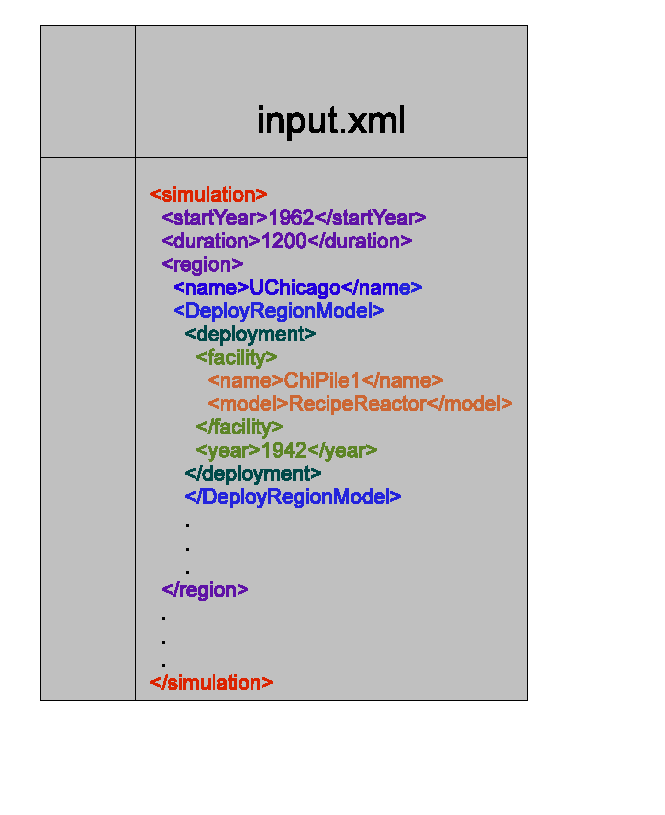
\includegraphics[height=5.5cm]{user.eps}
    \end{center}
    \caption { XML input parsing and a relaxNG schema provide 
    a simplified XML interface is available for the end
    user to define available module implementations of models and data. }
    \label{fig:xmlinput}
  \end{figure}

\end{frame}

%||||---------------
\begin{frame}[ctb!]
  \frametitle{Version Control}
    This open source repository employs a version control system 
     for provenance, developer access, and reproducibility of results.
  \begin{figure}[htbp!]
    \begin{center}
      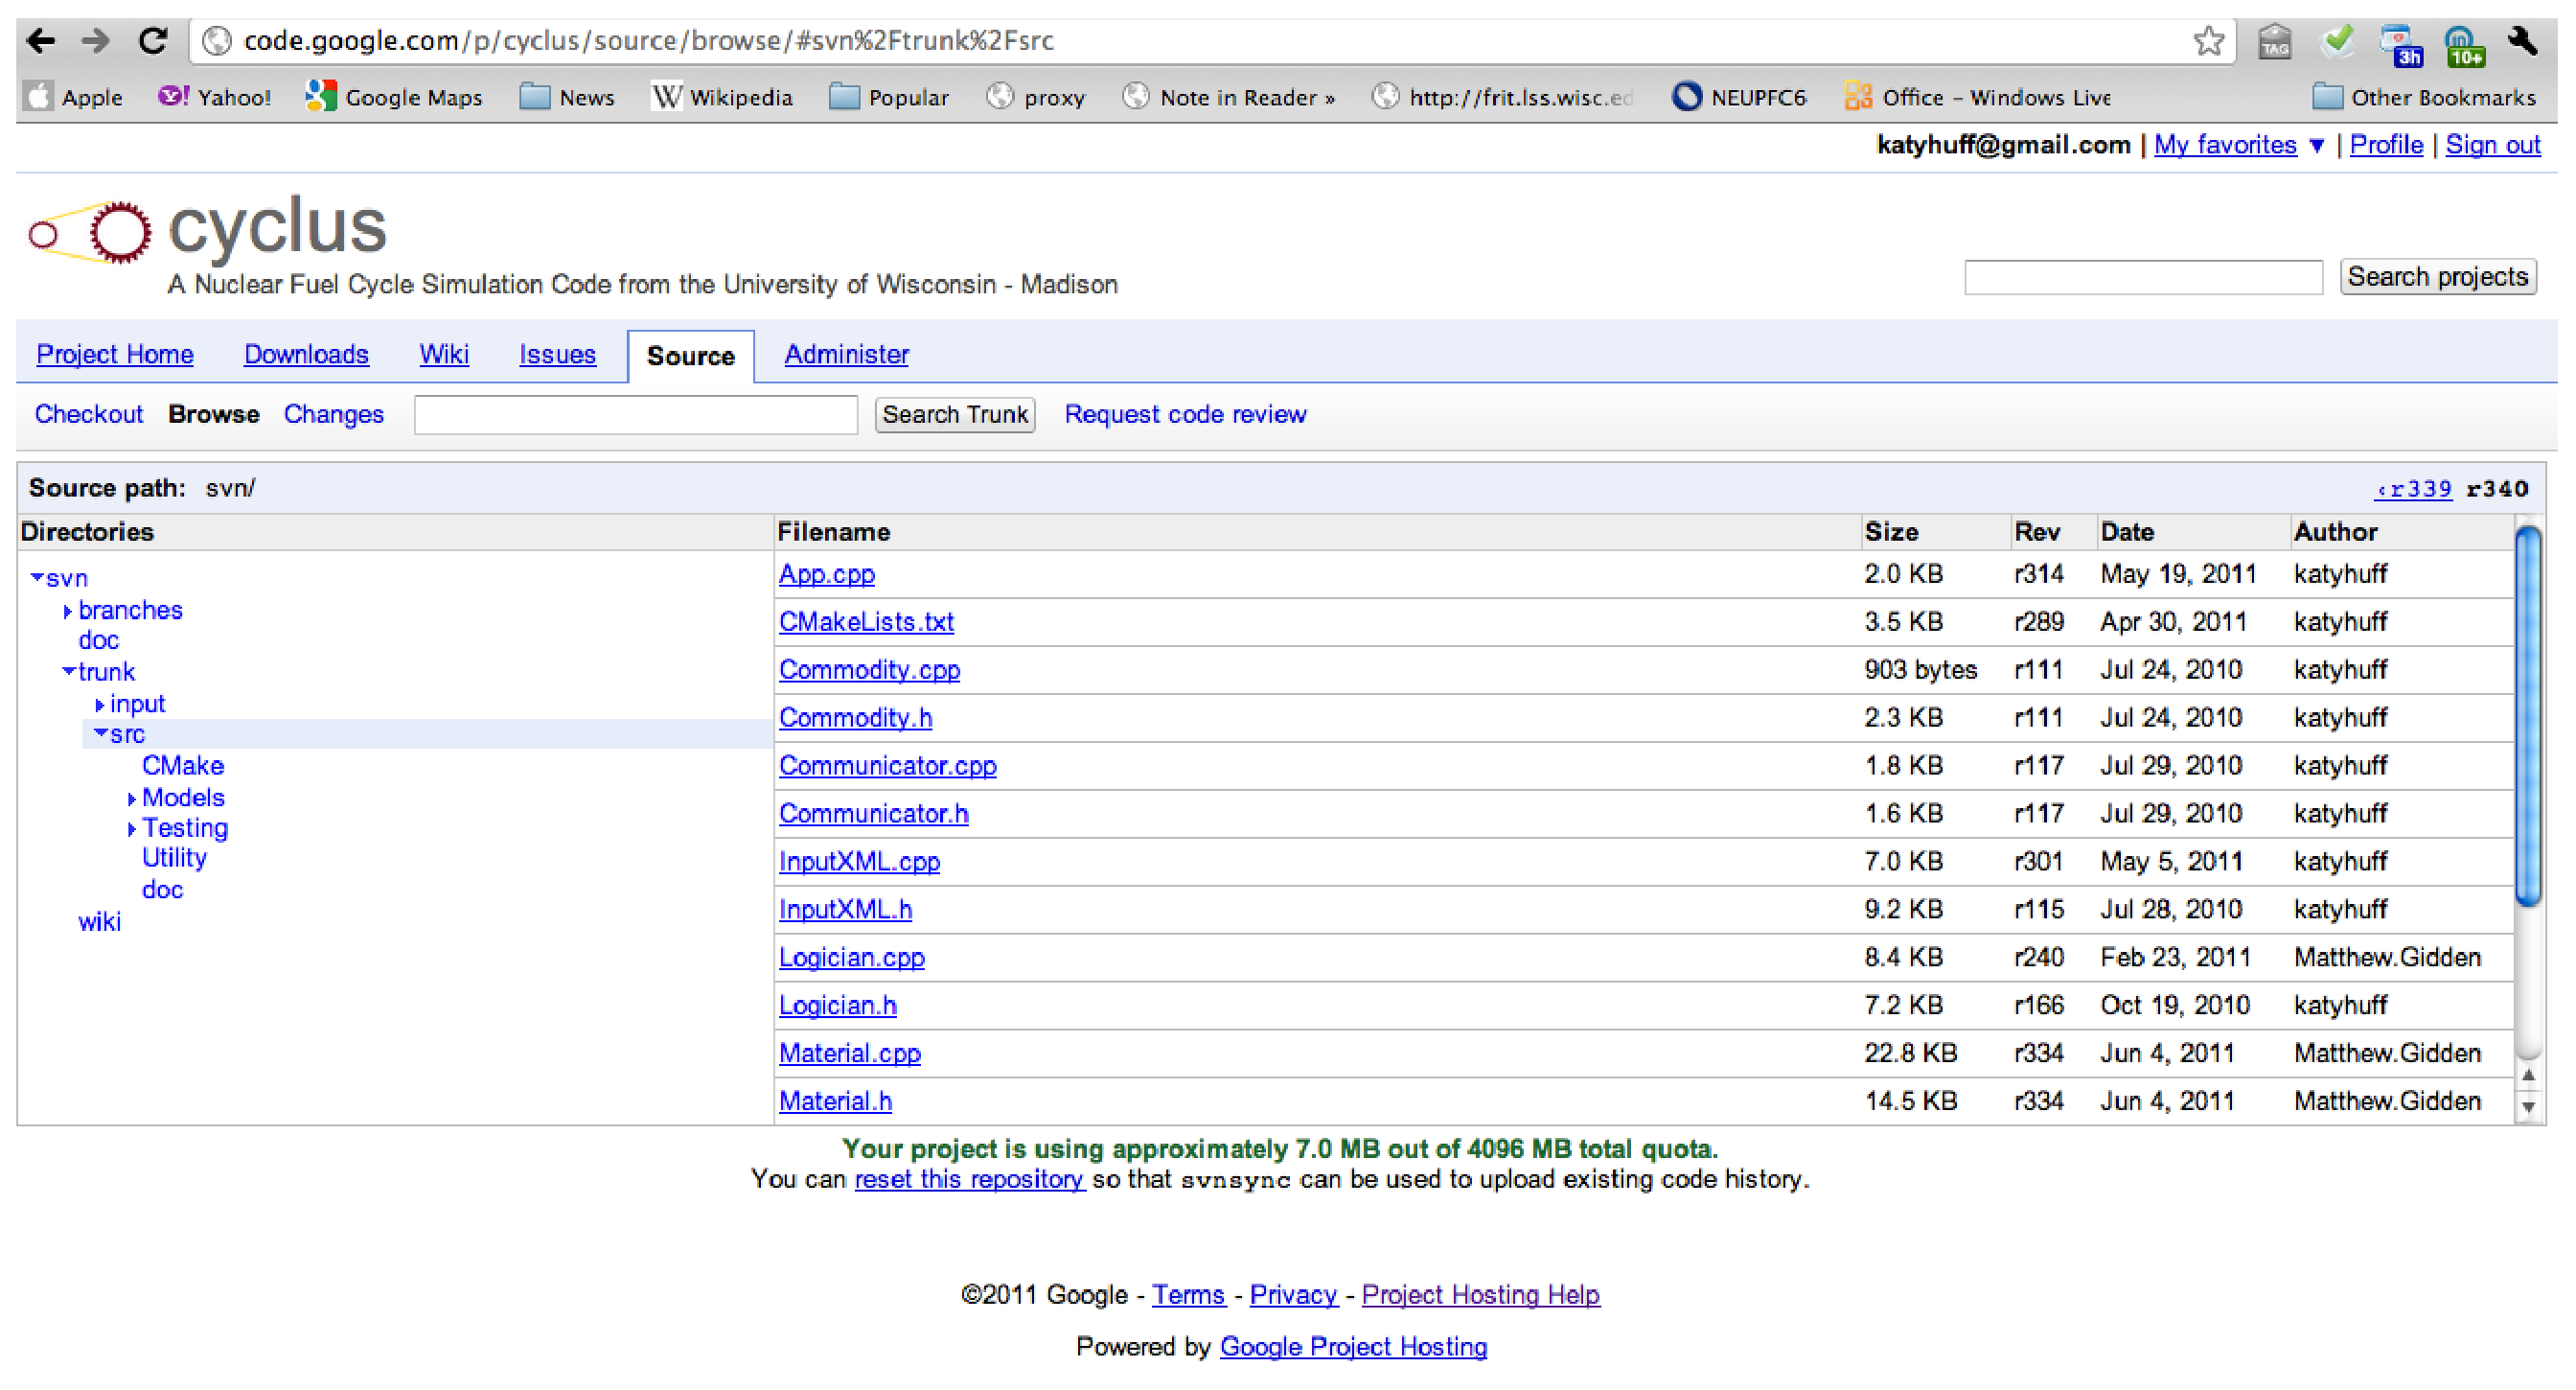
\includegraphics[height=6cm]{source.eps}
    \end{center}
    \caption{The current source code, tests, commit messages, and complete 
    revision history are recorded and available in the repository.}
    \label{fig:source}
  \end{figure}
\end{frame}

